% Paquets généraux
\documentclass[a4paper,12pt,titlepage]{article}
\usepackage[T1]{fontenc}
\usepackage[utf8]{inputenc}
\usepackage[french]{babel}
\usepackage[gen]{eurosym}
%\usepackage[dvips]{graphicx}
\usepackage{fancyhdr}
\usepackage{pdfpages} 
\usepackage{multido}
\usepackage{hyperref}
%\usepackage{textcomp}
%\usepackage{aeguill}
\usepackage{schemabloc}
\usepackage[bitstream-charter]{mathdesign}
\usepackage{minted}

\newcommand{\id}{71}
\newcommand{\nom}{Théorie des mécanismes}
\newcommand{\sequence}{04}
\newcommand{\nomsequence}{Liaisons entre les solides}
\newcommand{\num}{02}
\newcommand{\type}{KH}
\newcommand{\descrip}{Liaisons équivalentes, hyperstatisme, liaisons en série et en parallèle, théorie des graphes}
\newcommand{\competences}{B2-12: Proposer une modélisation des liaisons avec leurs caractéristiques géométriques. \\ &  B2-13: Proposer un modèle cinématique paramétré à partir d'un système réel, d'une maquette numérique ou d'u \\ &  B2-17: Simplifier un modèle de mécanisme. \\ &  B2-18: Modifier un modèle pour le rendre isostatique. \\ &  C1-04: Proposer une démarche permettant d'obtenir une loi entrée-sortie géométrique.  \\ &  C2-05: Caractériser le mouvement d'un repère par rapport à un autre repère. \\ &  C2-06: Déterminer les relations entre les grandeurs géométriques ou cinématiques. }
\newcommand{\nbcomp}{7}
\newcommand{\systemes}{}
\newcommand{\systemesnum}{}
\newcommand{\systemessansaccent}{}
\newcommand{\ilot}{2}
\newcommand{\ilotstr}{02}
\newcommand{\dossierilot}{\detokenize{Ilot_02 }}


\newcommand{\auteurun}{Renaud Costadoat}
\newcommand{\auteurdeux}{Françoise Puig}
\newcommand{\institute}{Lycée Dorian}


\usepackage{color}
\usepackage{xcolor}
\usepackage{colortbl}
\usepackage{helvet}
\usepackage[frenchmath]{newtxsf} % for sans serif symbols
\renewcommand{\familydefault}{\sfdefault}
%\usepackage{amsfonts}
%\usepackage{amsmath}
%\usepackage{lmodern}
\usepackage{mathastext}
%\usepackage{xspace}
\usepackage{varioref}
\usepackage{tabularx}
%\usepackage{floatflt}
\usepackage{graphics}
\usepackage{wrapfig}
\usepackage{textcomp}
\usepackage{tikz}
\usepackage{wrapfig}
\usepackage{gensymb}
\usepackage[european]{circuitikz}
\usetikzlibrary{babel}
\usepackage{ifthen}
\usepackage{cancel}
\usepackage{etoolbox}
\usepackage{multirow}
%\usepackage{boxedminipage}
\definecolor{gris25}{gray}{0.75}
\definecolor{bleu}{RGB}{18,33,98}
\definecolor{bleuf}{RGB}{42,94,171}
\definecolor{bleuc}{RGB}{231,239,247}
\definecolor{rougef}{RGB}{185,18,27}
\definecolor{rougec}{RGB}{255,188,204}%255,230,231
\definecolor{vertf}{RGB}{103,126,82}
\definecolor{vertc}{RGB}{220,255,191}
\definecolor{forestgreen}{rgb}{0.13,0.54,0.13}
\definecolor{blcr}{rgb}{0.59,0.69,0.84}
\definecolor{blfr}{rgb}{0.32,0.51,0.75}
\definecolor{orfr}{rgb}{0.90,0.42,0.15}
\definecolor{orcr}{rgb}{0.90,0.65,0.50}
\definecolor{orangef}{rgb}{0.659,0.269,0.072}
\definecolor{orange}{rgb}{0.58,0.35,0.063}
\definecolor{orangec}{rgb}{0.43,0.32,0.25}
\definecolor{rcorrect}{rgb}{0.6,0,0}
\definecolor{sequence}{rgb}{0.75,0.75,0.75}
\definecolor{competences}{rgb}{0.61,0.73,0.35}
\definecolor{grisf}{HTML}{222222}
\definecolor{grisc}{HTML}{636363}
\definecolor{normal}{HTML}{4087c4}
\definecolor{info}{HTML}{5bc0de}
\definecolor{success}{RGB}{92,184,92}
\definecolor{warning}{RGB}{240,173,78}
\definecolor{danger}{RGB}{217,83,79}
\hypersetup{                    % parametrage des hyperliens
    colorlinks=true,                % colorise les liens
    breaklinks=true,                % permet les retours à la ligne pour les liens trop longs
    urlcolor= blfr,                 % couleur des hyperliens
    linkcolor= orange,                % couleur des liens internes aux documents (index, figures, tableaux, equations,...)
    citecolor= forestgreen                % couleur des liens vers les references bibliographiques
    }

% Mise en page
\pagestyle{fancy}

\setlength{\hoffset}{-18pt}

\setlength{\oddsidemargin}{0pt} 	% Marge gauche sur pages impaires
\setlength{\evensidemargin}{0pt} 	% Marge gauche sur pages paires
\setlength{\marginparwidth}{00pt} 	% Largeur de note dans la marge
\setlength{\headwidth}{481pt} 	 	% Largeur de la zone de tête (17cm)
\setlength{\textwidth}{481pt} 	 	% Largeur de la zone de texte (17cm)
\setlength{\voffset}{-18pt} 		% Bon pour DOS
\setlength{\marginparsep}{7pt}	 	% Séparation de la marge
\setlength{\topmargin}{-30pt} 		% Pas de marge en haut
\setlength{\headheight}{35pt} 		% Haut de page
\setlength{\headsep}{20pt} 		% Entre le haut de page et le texte
\setlength{\footskip}{30pt} 		% Bas de page + séparation
\setlength{\textheight}{700pt} 		% Hauteur de l'icone zone de texte (25cm)
\setlength\fboxrule{1 pt}
\renewcommand{\baselinestretch}{1}
\setcounter{tocdepth}{1}
\newcommand{\cadre}[2]
{\fbox{
  \begin{minipage}{#1\linewidth}
   \begin{center}
    #2\\
   \end{center}
  \end{minipage}
 }
}

\newcounter{num_quest} \setcounter{num_quest}{0}
\newcounter{num_rep} \setcounter{num_rep}{0}
\newcounter{num_cor} \setcounter{num_cor}{0}

\newcommand{\question}[1]{\refstepcounter{num_quest}\par
~\ \\ \parbox[t][][t]{0.15\linewidth}{\textbf{Question \arabic{num_quest}}}\parbox[t][][t]{0.93\linewidth}{#1}\par
}


\newcommand{\reponse}[1]
{\refstepcounter{num_rep}
\noindent
\rule{\linewidth}{.5pt}
\textbf{Question \arabic{num_rep}:}
\multido{\i=1+1}{#1}{~\ \\}
}

\newcommand{\cor}
{\refstepcounter{num_cor}
\noindent
\rule{\linewidth}{.5pt}
\textbf{Question \arabic{num_cor}:} \\
}

\newcommand{\titre}[1]
{\begin{center}
\cadre{0.8}{\huge #1} 
\end{center}
}


% En tête et pied de page
\fancypagestyle{normal}{%
  \fancyhf{}
\lhead{\nom}
\rhead{
\includegraphics[width=2cm]{../../img/logo}\hspace{2pt}}
\ifdef{\auteurdeux}{\lfoot{\auteurun,\auteurdeux}}{\lfoot{\auteurun}}
\cfoot{Page \thepage}}

\fancypagestyle{correction}{%
  \fancyhf{}
  \lhead{\colorbox{danger}{\begin{minipage}{0.65\paperwidth} \textcolor{white}{\textbf{Correction}} \end{minipage}} }
  \rhead{
\includegraphics[width=2cm]{../../img/logo}}
  \ifdef{\auteurdeux}{\lfoot{\auteurun,\auteurdeux}}{\lfoot{\auteurun}}
  \rfoot{\colorbox{danger}{\begin{minipage}{0.5\paperwidth} \begin{flushright}\textcolor{white}{\textbf{Correction}}\end{flushright} \end{minipage}} }}

\renewcommand{\footrulewidth}{0.4pt}

\usepackage{eso-pic}
\newcommand{\BackgroundPic}{%
\put(0,0){%
\parbox[b][\paperheight]{\paperwidth}{%
\vfill
\begin{center}
\hspace{0.5cm}\vspace{0.5cm}

\includegraphics[width=\paperwidth,height=\paperheight,%
keepaspectratio]{../../img/fond3}%
\end{center}
\vfill
}}}

\newcommand{\BackgroundPicdeux}{%
\put(25,-30){%
\parbox[b][\paperheight]{\paperwidth}{%
\vfill
\begin{center}

\includegraphics[width=\paperwidth,height=\paperheight,%
keepaspectratio]{../../img/fond4}%
\end{center}
\vfill
}}}

\begin{document}

\pagestyle{empty}

\vspace*{-3\baselineskip}

\AddToShipoutPicture*{\BackgroundPic}

\ifdef{\auteurdeux}{\begin{tabular}{>{\columncolor{gray!00}}m{.3\linewidth} m{.3\linewidth} >{\columncolor{gray!00}}m{.3\linewidth}}
Séquence : \sequence &  \multirow{3}{*}{\hspace{1cm}
\includegraphics[height=1.5cm]{../../img/logo}} &  \begin{flushright} \multirow{4}{*}{\hspace{1cm}\includegraphics[height=4cm]{img/qrcode}}\end{flushright}\\
Document : \type\num \\
 \institute \\
 \auteurun\\
 \auteurdeux
\end{tabular}}{\begin{tabular}{>{\columncolor{gray!00}}m{.3\linewidth} m{.3\linewidth} >{\columncolor{gray!00}}m{.3\linewidth}}
Séquence : \sequence &  \multirow{3}{*}{\hspace{1cm}
\includegraphics[height=1.5cm]{../../img/logo}} &  \begin{flushright} \multirow{4}{*}{\hspace{1cm}\includegraphics[height=4cm]{img/qrcode}}\end{flushright}\\
Document : \type\num \\
 \institute \\
 \auteurun
\end{tabular}}

\vspace{1cm}

\ifdef{\prive}{\begin{center}\colorbox{danger}{\Huge{Avec Correction}}\end{center}}{}

\begin{center}\huge{\nom}\end{center}

\vspace{2cm}

\ifdef{\imagedeux}{\begin{minipage}{0.49\linewidth}}{}
\begin{center}\includegraphics[height=5cm]{/home/renaud/Documents/Renaud/GitHub/django_education/systemes/\imageun}\end{center}
\ifdef{\imagedeux}{\end{minipage}\hfill
\begin{minipage}{0.49\linewidth}
\begin{center}\includegraphics[height=5cm]{/home/renaud/Documents/Renaud/GitHub/django_education/systemes/\imagedeux}\end{center}
\end{minipage}}{}

\vspace{5cm}


\begin{tabular}{p{.15\linewidth} >{\columncolor{white}}p{.8\linewidth}}
    \rowcolor{gray!20}
    Référence & S\sequence\ - \type\num \\
    Compétences & \competences \\
 	\rowcolor{gray!20}
    Description & \descrip \\
    Système & \systemes
  \end{tabular}

\newpage

\AddToShipoutPicture{\BackgroundPicdeux}

\pagestyle{normal}

\section{Présentation du système étudié}

Le système utilisé est un pilote automatique pour voilier. En pilotage manuel, lorsque le barreur désire suivre un cap, il doit constamment utiliser les informations données par le compas et corriger l'orientation du safran en fonction de l'écart constaté entre le cap désiré et le cap réel. Le barreur doit aussi pouvoir intervenir sur le réglage des voiles. C'est pourquoi le pilote automatique doit alors permettre au barreur d'assurer la prise en charge du cap lorsqu'il doit se consacrer à d'autres tâches. 
Le pilote automatique est constitué de:
\begin{itemize}
 \item une unité de calcul AC10 et d'une console d'affichage et de saisie AP16,
 \item un moteur à courant continu,
 \item une pompe à pistons axiaux,
 \item un by-pass,
 \item un vérin hydraulique double tige,
 \item un bras de mèche solidaire au safran,
 \item un capteur angulaire.
\end{itemize}

\begin{figure}[h!]
 \begin{minipage}{0.49\linewidth}
\centering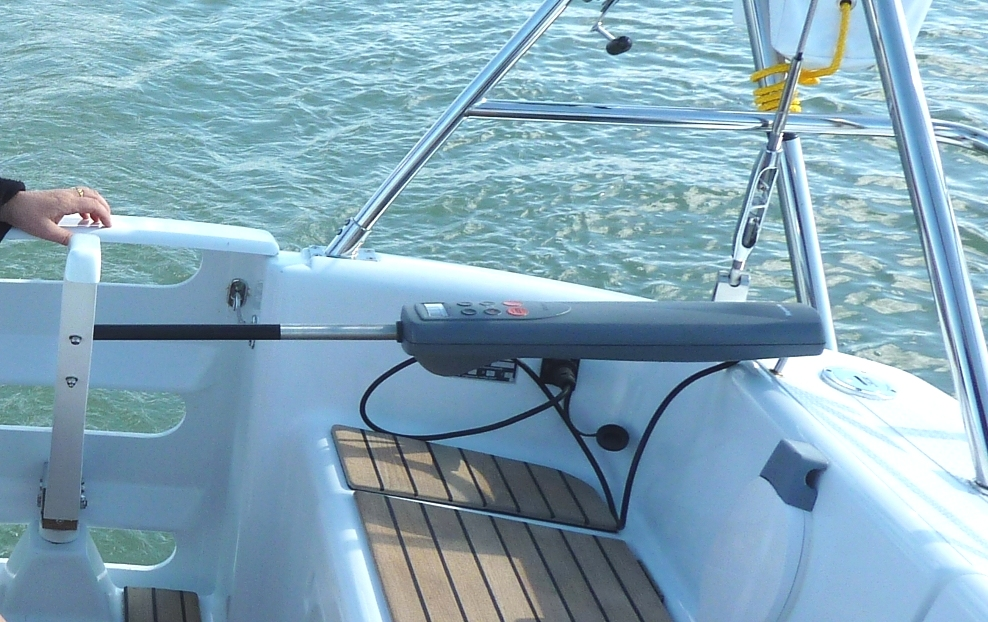
\includegraphics[width=0.8\linewidth]{img/pilote1.jpg}
\caption{Pilote installé}
\end{minipage}
 \hfill
  \begin{minipage}{0.49\linewidth}
\centering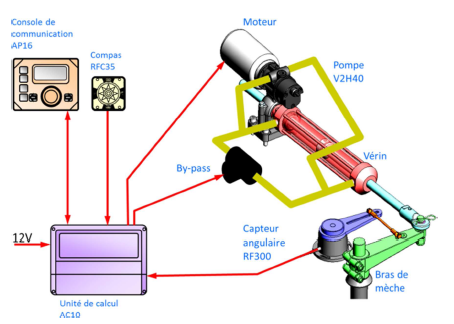
\includegraphics[width=0.8\linewidth]{img/pilote.png}
\caption{Schéma du pilote}
 \end{minipage}
\end{figure}

Ce TD s'intéresse à la fabrication du corps et du carter de la pompe. Plusieurs évolutions de cette pompe ont mené aux changements successifs de son procédé d'obtention. Dans un premier temps, le brut est obtenu par moulage au sable. Le carter est quant à lui obtenu en injection plastique.

\section{Moulage en sable du corps de pompe}

\subsection{Etude des matériaux adaptés au moulage au sable}

\paragraph{Question 1:} Le corps de pompe est en FGS 250. Expliciter cette désignation.

\paragraph{Question 2:} Préciser sa température de fusion, sa résistance élastique ainsi que des exemples d'application.

Dans le but de mouler des parties creuses, un noyau peut être utilisé.

\paragraph{Question 3:} Quel est le matériau utilisé pour la fabrication des noyaux.

Justifier ce choix.

\subsection{Etude du procédé de moulage au sable}

Mise en \oe uvre du procédé, observation de la pièce exemple.

\paragraph{Question 4:} Expliquer en quoi le moulage en sable est un procédé à \og moule non permanent à modèle permanent \fg.

\paragraph{Question 5:} Quels sont les éléments nécessaires à la coulée ?

Quel est le rôle des masselottes ? Des évents ?

A quoi servent les étapes de sciage et d'ébarbage ?

Quel est le rôle des noyaux ? Quel est leur procédé de fabrication ?

Quel est le rôle des dépouilles?

\paragraph{Question 6:} Evaluer l'épaisseur moyenne de la pièce.

\paragraph{Question 7:} Comment expliquer la nécessité d'avoir des épaisseurs constantes ?

Les surépaisseurs d'usinage sont de 1mm.

Les épaisseurs données sont-elles compatibles avec les données fournies dans le tableau ci-après ?

Si cela ne correspond pas quel peut être le problème?


\begin{table}[!h]
\begin{center}
\scalebox{0.7}{
\begin{tabular}{|c|c|c|c|c|c|}
\hline
Matériau & Fonte moulée & Acier moulé & Alliage d'alu. & Alliage d'alu. & Alliage d'alu. \\
et procédé & au sable & au sable & moulé au sable & moulé en coquille & moulé en coquille  \\
 &  &  & & par gravité & sous pression \\
\hline
Surépaisseur & $2.5mm$ & $4mm$ & $2mm$ & $(1+4.5.10^{-3}.L)mm$ & $0.3mm$ \\
 mini &  & & & & \\
\hline
\end{tabular}}
\end{center}
\end{table}

\subsection{Représentation de la pièce moulée et des éléments permettant le moulage}

\paragraph{Question 8:} Indiquer et tracer sur le dessin prévu à cet effet :

\begin{figure}[!h]
 \begin{minipage}{0.49\linewidth}
\begin{enumerate}
\item En noir :
 \begin{itemize}
  \item Le plan de joint,
  \item Les deux parties du moule et les châssis.
 \end{itemize}
 \item En bleu :
 \begin{itemize}
  \item Le trou de coulée,
  \item Le chenal d'alimentation,
  \item Les masselottes, les évents.
 \end{itemize}
\end{enumerate}
 \end{minipage}
 \hfill
  \begin{minipage}{0.49\linewidth}
\begin{enumerate}
\setcounter{enumi}{2}
 \item En vert :
 \begin{itemize}
  \item Le noyau,
  \item Les portées de noyau.
 \end{itemize}
 \item En rouge :
 \begin{itemize}
  \item Les surépaisseurs d'usinage,
  \item Les dépouilles.
 \end{itemize}
\end{enumerate}
 \end{minipage}
\end{figure}


\section{Injection plastique du boitier de pompe}

L'injection plastique peut être vue comme un procédé équivalent au moulage en coquille utilisé pour les matériaux métalliques.

\subsection{Etude du procédé de moulage en injection plastique}

Le boitier de pompe est en polycarbonate.

\paragraph{Question 9:} De quelle famille de matériaux s'agit-il ?

Mise en \oe uvre du procédé

\paragraph{Question 10:} Dans le cadre de l'injection plastique comment est réalisée la fonte du plastique ?

Qu'est-ce que le \og poteyage \fg ?

Existe-t-il des opérations de parachèvement ?

\paragraph{Question 11:} Quel est le coût du procédé de moulage en coquille ? Comment expliquer la différence avec le coût du moulage en sable ?

\paragraph{Question 12:} Proposer des solutions permettant le taraudage de la pièce.

\paragraph{Question 13:} Soit une pièce moulée en sable et une pièce injectée, laquelle aura les plus grands rayons de raccordement ? Pourquoi ?

\subsection{Représentation des éléments associés au moulage en coquille}

\paragraph{Question 14:} En considérant que le boîtier est réalisé en moulage en coquille par gravité, indiquer et tracer sur le dessin prévu à cet effet :
\begin{figure}[!h]
 \begin{minipage}{0.49\linewidth}
\begin{enumerate}
 \item En noir :
 \begin{itemize}
  \item Le plan de joint,
  \item La semelle,
  \item Les chapes,
  \item La broche,
  \item Le système d'éjection.
 \end{itemize}
\end{enumerate}
 \end{minipage}
 \hfill
  \begin{minipage}{0.49\linewidth}
\begin{enumerate}
\setcounter{enumi}{1}
 \item En bleu
 \begin{itemize}
  \item Les dépouilles
 \end{itemize}
\end{enumerate}
 \end{minipage}
\end{figure}

\section{Moulage en coquille}

Cette partie est à réaliser à partir de vos connaissances et en dehors du contexte de l'exercice.

\paragraph{Question 15:} Dans le tableau de synthèse, remplir la 3ème colonne (Moulage en coquille). Il faudra préciser, en particulier :
L'épaisseur moyenne, la surépaisseur d'usinage et la rugosité,
Le matériau et sa température de fusion.

\section{Synthèse des procédés de moulage}
\paragraph{Question 16:} Sur le document réponse, réaliser la comparaison du moulage en coquille, du moulage au sable et de l'injection plastique.

La fonte est-elle utilisable en moulage en coquille ? Si non, pourquoi ?

Compléter alors le tableau de synthèse.

\newpage

\begin{figure}[!h]
 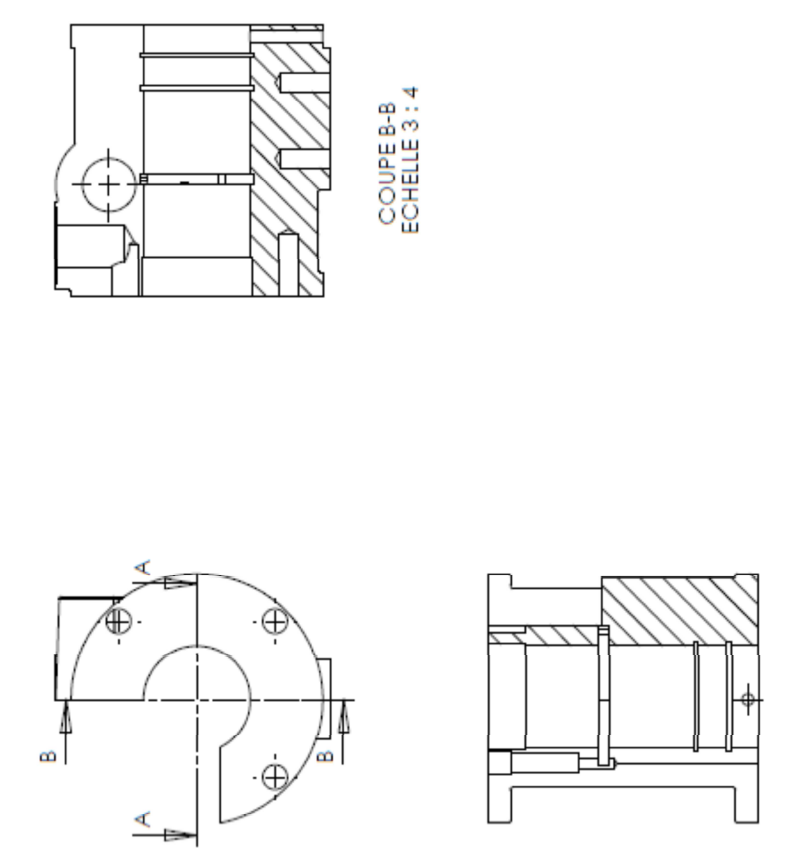
\includegraphics[width=0.9\linewidth]{img/dessin1.png}
 \caption{Document réponse 1 : Corps de pompe}
\end{figure}

\newpage

\begin{figure}[!h]
 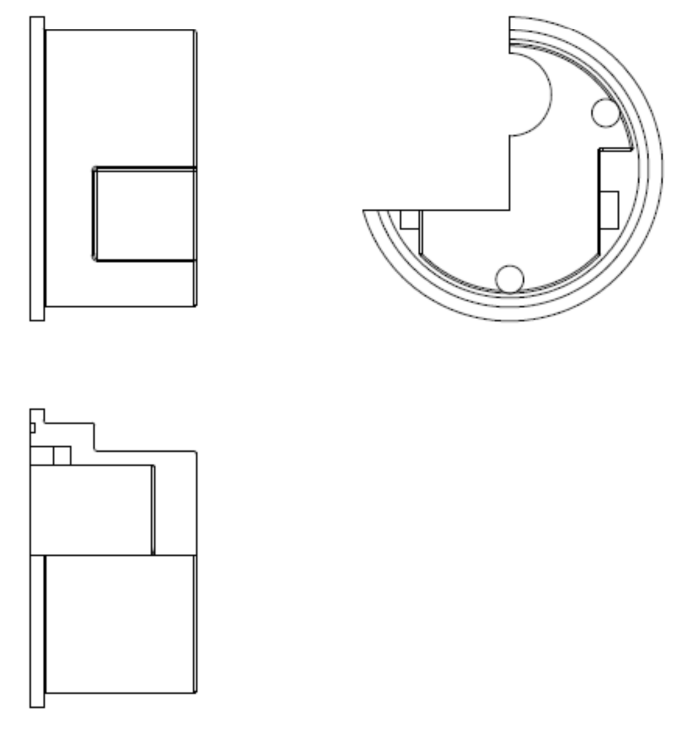
\includegraphics[width=0.9\linewidth]{img/dessin2.png}
 \caption{Document réponse 2 : Boitier}
 \end{figure}

\newpage

\begin{table}[!h]
\begin{center}
\scalebox{0.7}{
\begin{tabular}{|c|c|c|c|}
\hline
 & Moulage en sable & Moulage en coquille & Injection plastique \\
 \hline
\textbf{Procédé} & & & \\
Surépaisseur d'usinage  & & & \\
Rugosité  & & & \\
Epaisseur minimale  & & & \\
Tolérances du brut  & & & \\
Arrondi (++, +, - ou --)  & & & \\
 & & & \\
 & & & \\
 & & & \\
 & & & \\
 & & & \\
 & & & \\
 & & & \\
 & & & \\
 & & & \\
 & & & \\
\hline
\textbf{Produit}  & & & \\
Série  & & & \\
Formes  & & & \\
Tailles  & & & \\
 & & & \\
 & & & \\
 & & & \\
 & & & \\
 & & & \\
 & & & \\
 & & & \\
 & & & \\
 & & & \\
 & & & \\
\hline
\textbf{Matériaux}  & & & \\
(Indiquer la désignation)  & & & \\
Alliage ferreux (Fontes)  & & & \\
Alliage non ferreux  & & & \\
Polymère et/ou élastomère  & & & \\
 & & & \\
 & & & \\
 & & & \\
 & & & \\
 & & & \\
 & & & \\
 & & & \\
 & & & \\
 & & & \\
 & & & \\
\hline
\end{tabular}}
\end{center}
\end{table}

\newpage

\section{Conception d'un corp d'affuteuse}

L'aiguisage consiste à donner ou rendre à une lame un tranchant utile. Il doit être effectué une fois à la fabrication de l'outil, puis régulièrement par l'utilisateur, afin de la garder tranchante.

\begin{figure}[!h]
 \begin{minipage}{0.45\linewidth}
Une affuteuse est une machine, qui sert à rendre un ou plusieurs outils plus tranchants ou plus pointus.
\end{minipage}
\hfill
 \begin{minipage}{0.5\linewidth}
  \centering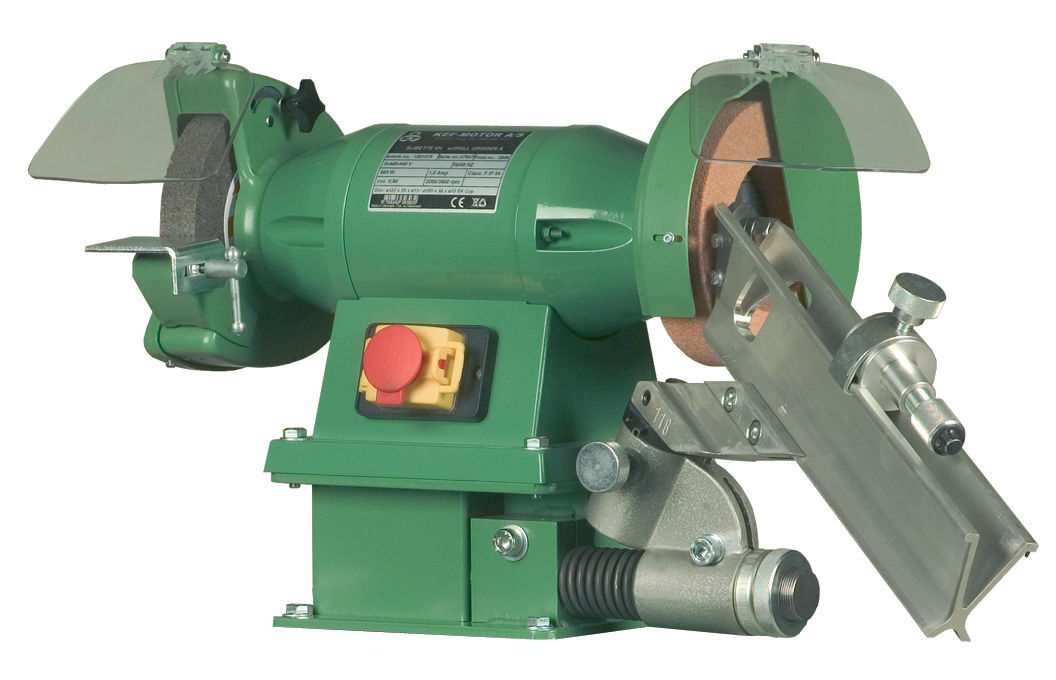
\includegraphics[width=1\linewidth]{img/affuteuse.jpg}
  \caption{Affuteuse électrique}
  \label{img:image4}
 \end{minipage}
\end{figure}

Le corp de l'affuteuse est la pièce (verte sur la figure \ref{img:image4}) qui permet:
\begin{itemize}
 \item de guider l'arbre en rotation (grâce à des roulements à bille),
 \item de fixer l'affuteuse à son support. 
\end{itemize}

L'objectif de cet exercice est de définir la géométrie volumique de cette pièce. Les contraintes sont les suivantes:
\begin{itemize}
 \item Les surfaces fonctionnelles d'un corp d'affuteuse sont données,
 \item Le procédé de fabrication choisi est le moulage en sable.
\end{itemize}

\textit{Remarque:} Le fait que le procédé de mise en forme du brut soit le moulage impose des règles de tracé pour celui-ci.

\paragraph{Question 1:} Dessiner sur le document réponse un solution pour la géométrie de la pièce support.

\paragraph{Question 2:} Ajouter les éléments nécessaires à la définition du moule sur le dessin.


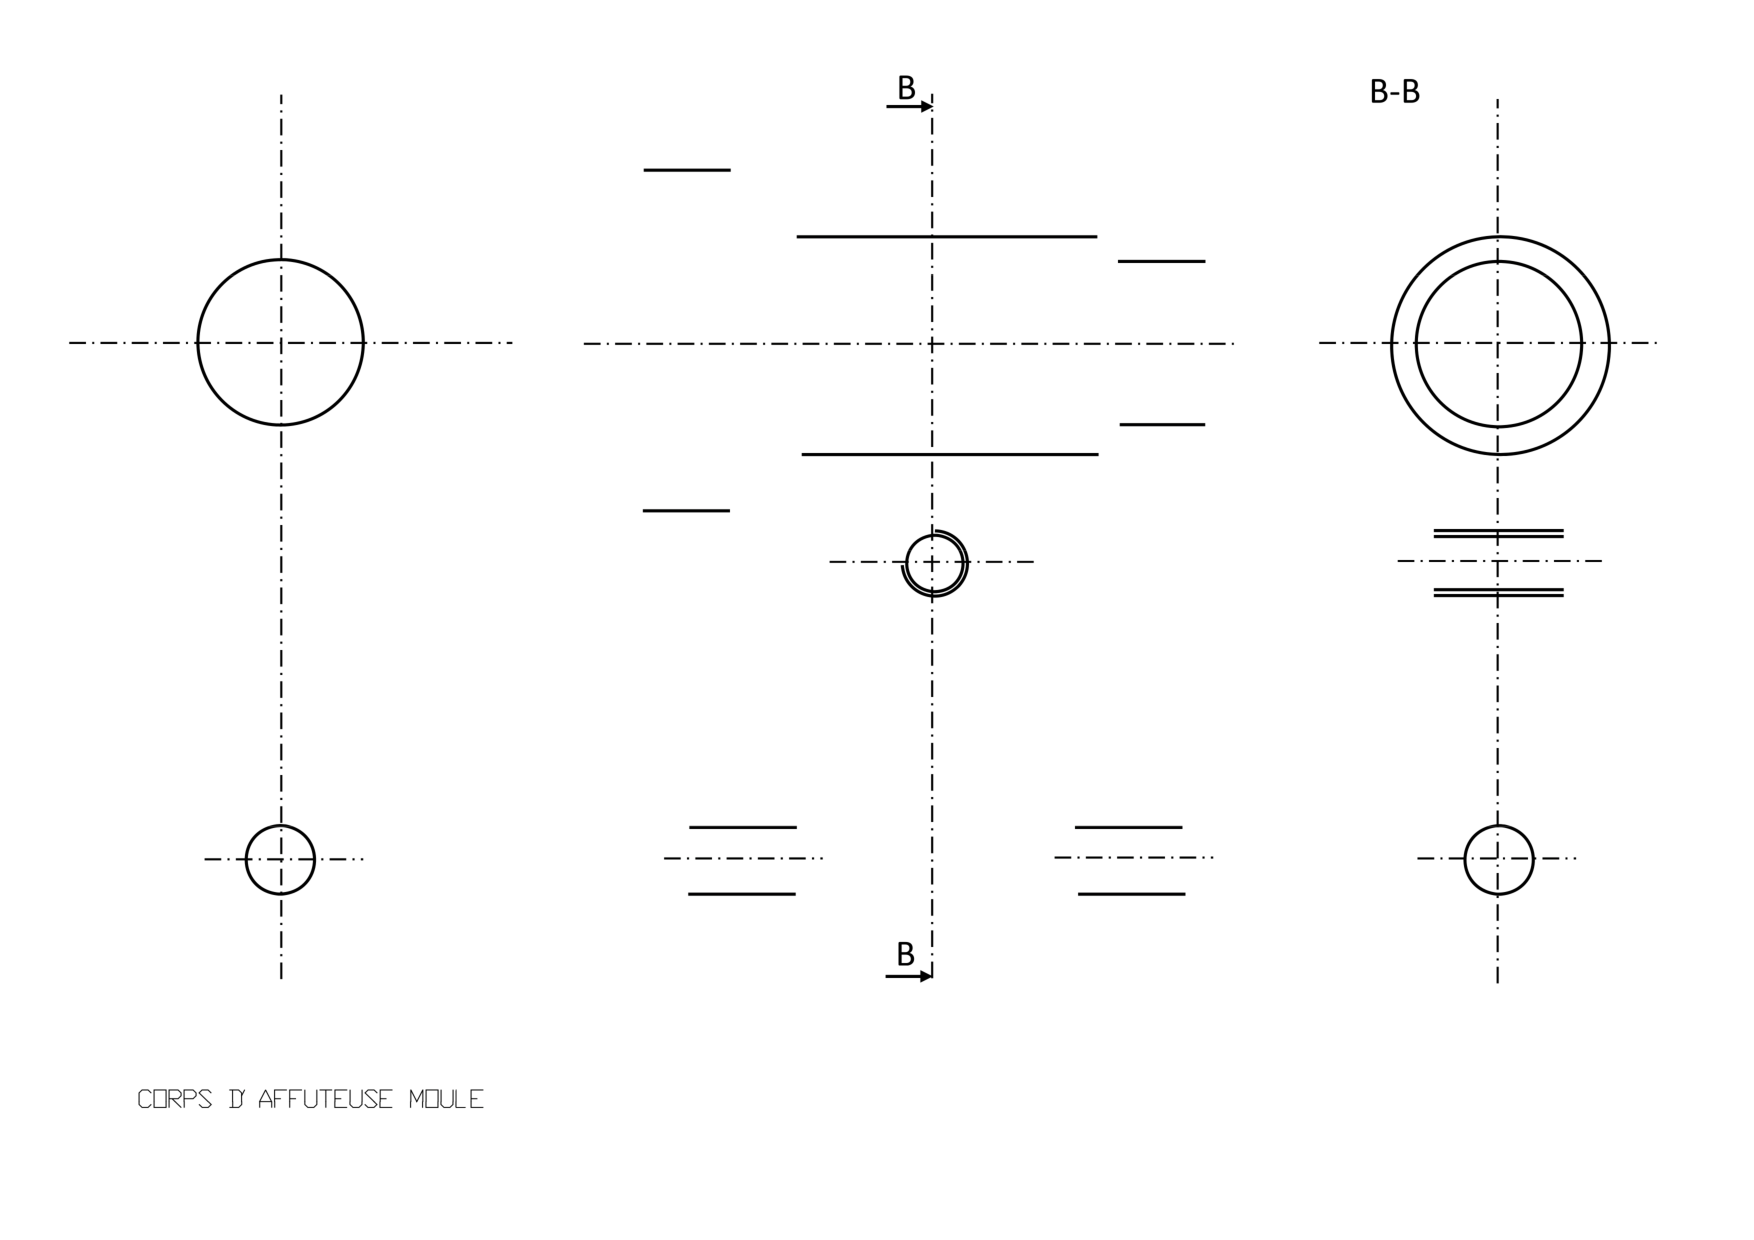
\includepdf[landscape=true]{img/Corp_affuteuse.pdf}
\clearpage

\ifdef{\public}{\end{document}}{}

\newpage

\pagestyle{correction}

\section{Correction}


\end{document}